\documentclass[10pt,table]{beamer}
\usepackage[utf8]{luainputenc}
\usepackage[ngerman]{babel}


%\usetheme[block=fill]{m}                     % Use metropolis theme
\usepackage{beamerthemeuzl-conference}

\usepackage{Alegreya,AlegreyaSans}

\logo{
\includegraphics[scale=.62]{uzl-logo-ITCS.pdf}}
\usepackage{amsmath}
\DeclareMathOperator*{\argmin}{arg\,min}
\usepackage{nicefrac}
\usepackage{algorithm}
\usepackage{dsfont}
\usepackage{subfig}
\usepackage{mathtools}
\usepackage{graphicx}
\usepackage{mathpazo} 
\usepackage{tikz}

\usepackage{algorithm}
\usepackage{algorithmic}
\usepackage{xspace}
\usepackage{float}
\usepackage{subfig}
\usepackage{color, colortbl}
\definecolor{uzlred}{HTML}{BF0000}
\definecolor{uzlgreen}{HTML}{008000}
\definecolor{uzlpurple}{HTML}{700080}
\newcommand{\highlightrow}{\rowcolor{Ozeangruen!5}}

\newcommand{\km}{\varkappa}
\newcommand{\kmeans}{$\varkappa$\texttt{-means}\xspace}
\newcommand{\kmeansplusplus}{$\varkappa$\texttt{-means++}\xspace}

\newcommand{\kanonymeans}{\texttt{kAnonyMeans}\xspace}
\newcommand{\kanonymeansstar}{$\texttt{kAnonyMeans}^*$\xspace}

\newcommand{\sse}{\textsc{sse}\xspace}

\newcommand{\mdav}{\texttt{MDAV}\xspace}
\newcommand{\mdavplus}{$\mdav^+$\xspace}
\newcommand{\vmdav}{\texttt{V-MDAV}\xspace}
\newcommand{\mdavstar}{$\mdav^*$\xspace}

\newcommand{\mergeandsplit}{\texttt{MergeAndSplit}\xspace}
\newcommand{\merge}{\texttt{Merge}\xspace}
\newcommand{\splitx}{\texttt{Split}\xspace}

\newcommand{\forgy}{\texttt{Forgy}\xspace}

\title{Datenbankanonymisierung auf Basis von k-means-Algorithmen}
%\subtitle{}
\author{Finn Stoldt}
\date{19.12.2019}


\begin{document}
\maketitle


\iffalse
\begin{frame}{Überblick}
\tableofcontents[hideallsubsections]
\end{frame}

\AtBeginSection[]
{
  \begin{frame}
    \frametitle{Überblick}
    \tableofcontents[currentsection, hideallsubsections]
  \end{frame}
}
\fi

\AtBeginSection[]{
  \begin{frame}[noframenumbering]
  \vfill
  \centering
  \begin{beamercolorbox}[sep=8pt,center,shadow=true,rounded=true]{title}
    \usebeamerfont{title}\insertsectionhead\par%
  \end{beamercolorbox}
  \vfill
  \end{frame}
}

\section{Einleitung}
\begin{frame}{Einleitung}
    \begin{center}
         
\includegraphics[scale=0.1]{Images/netflixLogo.png}
    \end{center}
\end{frame}

\begin{frame}{Einleitung}
Netflix Prize dataset
\begin{itemize}
    \item 2006 veröffentlicht
    \item pseudonymisierte Filmbewertungen (mit Datum)
    \item von 500.000 Abonnenten
    \item Re-Identifizierung über öffentliche IMDb möglich
\end{itemize}
\end{frame}

\begin{frame}{Einleitung}
\begin{itemize}
    \item Pseudonymisierung garantiert keine Anonymität.
    \item Daten müssen \emph{anonymisiert} werden.
    \item Orientieren uns an Datenschutzmodell \emph{$k$-Anonymität}.
    \item Kann durch \emph{Mikroaggregation} erreicht werden.
\end{itemize}
\end{frame}

\section{Grundlagen}
\begin{frame}{Daten}
    Datenbank $\mathcal{X}\in\mathbb{R}^{n\times m}$ mit $n$ Elementen mit $m$ reellwertigen Quasi-Identifikatoren
    \\~\\
    $i$-tes Element repräsentiert durch Vektor $\mathbf{x}_i = (x_1,...,x_m)$
    \\~\\~\\
    \begin{columns}
        \begin{column}{0.42\textwidth}
            Abstand zwischen $\mathbf{x},\mathbf{x}^\prime\in\mathcal{X}$
            \begin{align*}
                d(\mathbf{x},\mathbf{x}^\prime) := \sum\limits_{i=1}^m(x_i-x^\prime_i)^2
            \end{align*}
            Abstand zwischen $\mathcal{X},\mathcal{X}^\prime\in\mathbb{R}^{n\times m}$
            \begin{align*}
                 \sse(\mathcal{X},\mathcal{X}^\prime) := \sum\limits_{i=1}^nd(\mathbf{x},\mathbf{x}^\prime)
            \end{align*}
        \end{column}
        \begin{column}{0.5\textwidth}
            Schwerpunkt von $\mathcal{X}\in\mathbb{R}^{n\times m}$
            \begin{align*}
                c(\mathcal{X}) := \frac{1}{|\mathcal{X}|}\sum\limits_{\mathbf{x}\in\mathcal{X}}\mathbf{x}
            \end{align*}
            Abstand zwischen allen $\mathbf{x}\in\mathcal{X}$ und $c(\mathcal{X})$
            \begin{align*}
                \sse(\mathcal{X}) := \sum\limits_{\mathbf{x}\in\mathcal{X}}d(\mathbf{x},c(\mathcal{X}))
            \end{align*}
        \end{column}
    \end{columns}    
\end{frame}

\begin{frame}{Anonymisierung}
    $\mathcal{X}$ ist \emph{$k$-anonym}, wenn jeder Vektor $\mathbf{x}\in\mathcal{X}$ mindestens $k$ mal in $\mathcal{X}$ vorkommt.
    \\~\\~\\
    Ein \emph{Anonymisierungsalgorithmus} $\mu$ ist eine Abbildung $\mu : \mathbb{R}^{n\times m} \rightarrow \mathbb{R}^{n\times m}$,
    \begin{align*}
        \mu : \mathcal{X} := \mathbf{x}_1,...,\mathbf{x}_n \mapsto \hat{\mathcal{X}} := \hat{\mathbf{x}}_1,...,\hat{\mathbf{x}}_n
    \end{align*}
    \\~\\~\\
    Anonymisierung von $\mathcal{X}$ durch \emph{Mikroaggregation}:
    \begin{enumerate}
        \item $k$-Clustering $\mathcal{C}$ von $\mathcal{X}$ erzeugen.
        \item Für alle $C\in\mathcal{C}$: Ersetze alle $\mathbf{x}\in C\subset\mathcal{X}$ durch $c(C)$
    \end{enumerate}
\end{frame}

\begin{frame}{Anonymisierung}
    \emph{Anonymisierungsverzerrung} bei Anonymisierung von $\mathcal{X}$ durch $\mu$
    \begin{flalign*}
        D_\mu(\mathcal{X}) &:= \sse(\mathcal{X},\mu(\mathcal{X})) = \sse(\mathcal{X},\hat{\mathcal{X}})    &
    \end{flalign*}
    ~\\
    \emph{Diversität} von $\mathcal{X}$
    \begin{flalign*}
        \Delta(\mathcal{X}) &:= \sse(\mathcal{X})  &
    \end{flalign*}
    ~\\
    \emph{Informationsverlust} bei Anonymisierung von $\mathcal{X}$ durch $\mu$
    \begin{flalign*}
        L_\mu(\mathcal{X}) &:=\frac{D_\mu(\mathcal{X})}{\Delta(\mathcal{X})}  &
    \end{flalign*}
\end{frame}

\begin{frame}{k-means}
    \begin{algorithm}[H]
    \renewcommand{\thealgorithm}{}
    \floatname{algorithm}{Algorithmus}
    \caption{\kmeans}
    \label{alg:kmeans}
    {\vspace*{0.1cm}
    \textbf{Eingabe:} Datenbank $\mathcal{X}$, Clusteranzahl $\km$ \\
    \textbf{Ausgabe:} Partition $\mathcal{C} = C_1,...,C_\km$ von $\mathcal{X}$
    \begin{enumerate}
    \item Wähle $\km$ beliebige Elemente aus $\mathcal{X}$ als Mittelpunkte $M = \mathbf{m}_1, ...,\mathbf{m}_\km$.
    \item Ordne jedem Punkt $\mathbf{x}\in\mathcal{X}$ ein Cluster $C_i$ mit $i \in \{1,...,\km\}$ zu, für das $d(\mathbf{x},\mathbf{m}_i)$ minimal ist.
    \item Aktualisiere $\mathbf{m}_i$ für alle $i \in \{1,...,\km\}$, sodass $\mathbf{m}_i$ der Gruppenschwerpunkt aller Punkte in $C_i$ ist: $\mathbf{m}_i = c(C_i)$.
    \item Wiederhole Schritt 2 und 3 solange, bis sich $\mathcal{C}$ nicht mehr verändert.
    \end{enumerate}
    }
    \end{algorithm}
\end{frame}

\section{kAnonyMeans}
\subsection{Idee}
\begin{frame}{Idee}
    \begin{algorithm}[H]
    \renewcommand{\thealgorithm}{}
    \floatname{algorithm}{Algorithmus}
    \caption{\kanonymeans}
    \label{alg:kanonymeans}
    {
    \textbf{Eingabe:} Datenbank $\mathcal{X}$, Anonymitätsparameter $k$, Initiale Clusteranzahl $\km$\\
    \textbf{Ausgabe:} $k$-anonyme Datenbank $\hat{\mathcal{X}}$
    \begin{enumerate}
        \item Partitioniere die gegebene Datenbank $\mathcal{X}$ mittels \kmeans in $\km$ Cluster.
        \item Verschmelze durch \texttt{Merge} jedes Cluster mit weniger als $k$ Elementen mit anderen Clustern.
        \item Teile mittels \texttt{Split} jedes Cluster mit $2k$ oder mehr Elementen in kleinere auf.
        %\item Ersetze alle Elemente in $\mathcal{X}$ mit dem Schwerpunkt ihrer zugeordneten Gruppe.
    \end{enumerate}
    }
    \end{algorithm}
\end{frame}

\begin{frame}{Merge}
    Verschiedene Reihenfolgen durch unterschiedlichen Aufbau von \merge:
    \begin{itemize}
        \item mit innerer Schleife
        \item mit äußerer Schleife
        \item ohne weitere Schleife
    \end{itemize}
    ~\\~\\
    Verschiedene Eignungsmaße für Verschmelzungskandidaten:
    \begin{itemize}
        \item Mittelpunktabstand
        \item \sse-Zuwachs
    \end{itemize}
\end{frame}

\begin{frame}{Split}
    $k$-Clusterings müssen erzeugt werden $\Rightarrow$ \mdavplus
    \\~\\
    Verwenden \mdavplus da
    \begin{itemize}
        %\item $k$-Clustering notwendig
        \item geringe Clustervarianzen
        \item wenige Elemente
    \end{itemize}
\end{frame}

\subsection{MergeAndSplit während k-means}
\begin{frame}{MergeAndSplit während k-means}
    \begin{figure}
        \centering
        \scalebox{0.6}{
        \begin{tikzpicture}[line width=1.2]
            
            \tikzset{
                cross/.pic = {
                \draw[rotate = 45] (-####1,0) -- (####1,0);
                \draw[rotate = 45] (0,-####1) -- (0, ####1);
                }
            }        
            
            \def\circlesize{0.15}
            \def\colorA{Ozeangruen}
            \def\colorB{uzlred}
            \def\colorC{uzlgreen}
            \def\colorAFill{Ozeangruen!20}
            \def\colorBFill{uzlred!20}
            \def\colorCFill{uzlgreen!20}
            
            \begin{scope}[xshift=-180]
                \draw[\colorA,fill=\colorAFill] (0,2.5) circle (\circlesize);
                \path[\colorA] (0,2.5) pic {cross=0.15};
            
                \draw[\colorB,fill=\colorBFill] (1,1) circle (\circlesize);
                \draw[\colorB,fill=\colorBFill] (1,-1) circle (\circlesize);
                \draw[\colorB,fill=\colorBFill] (-1,-1) circle (\circlesize);
                \draw[\colorB,fill=\colorBFill] (-1,1) circle (\circlesize);
                \path[\colorB] (0,0) pic {cross=0.15};
                
                \draw[\colorC,fill=\colorCFill] (0.4,-1.9) circle (\circlesize);
                \draw[\colorC,fill=\colorCFill] (-0.4,-1.9) circle (\circlesize);
                \draw[\colorC,fill=\colorCFill] (0,-2.4) circle (\circlesize);
                \path[\colorC] (0,-2.05) pic {cross=0.15}; 
            \end{scope}
            
            \begin{scope}
                \draw[\colorB,fill=\colorBFill] (0,2.5) circle (\circlesize);
            
                \draw[\colorB,fill=\colorBFill] (1,1) circle (\circlesize);
                \draw[\colorB,fill=\colorBFill] (1,-1) circle (\circlesize);
                \draw[\colorB,fill=\colorBFill] (-1,-1) circle (\circlesize);
                \draw[\colorB,fill=\colorBFill] (-1,1) circle (\circlesize);
                \path[\colorB] (0,0.5) pic {cross=0.15};
                
                \draw[\colorC,fill=\colorCFill] (0.4,-1.9) circle (\circlesize);
                \draw[\colorC,fill=\colorCFill] (-0.4,-1.9) circle (\circlesize);
                \draw[\colorC,fill=\colorCFill] (0,-2.4) circle (\circlesize);
                \path[\colorC] (0,-2.05) pic {cross=0.15}; 
            \end{scope}
            
            \begin{scope}[xshift=180]
                \draw[\colorB,fill=\colorBFill] (0,2.5) circle (\circlesize);
            
                \draw[\colorB,fill=\colorBFill] (1,1) circle (\circlesize);
                \draw[\colorB,fill=\colorBFill] (-1,1) circle (\circlesize);
                \path[\colorB] (0,1.5) pic {cross=0.15};
                
                \draw[\colorC,fill=\colorCFill] (1,-1) circle (\circlesize);
                \draw[\colorC,fill=\colorCFill] (-1,-1) circle (\circlesize);            
                \draw[\colorC,fill=\colorCFill] (0.4,-1.9) circle (\circlesize);
                \draw[\colorC,fill=\colorCFill] (-0.4,-1.9) circle (\circlesize);
                \draw[\colorC,fill=\colorCFill] (0,-2.4) circle (\circlesize);
                \path[\colorC] (0,-1.64) pic {cross=0.15}; 
            \end{scope}
            
            \draw[->, line width=0.5] (-4.6,0) -- node [above] {\texttt{MergeAndSplit}} (-1.9,0);
            \draw[->, line width=0.5] (1.9,0) -- node [above] {$\varkappa$-\texttt{means}} (4.6,0);
            
        \end{tikzpicture}
        }
        \caption{Beispiel-Situation für $k=3$ in der es sinnvoll ist, nach \mergeandsplit wieder \kmeans auszuführen. Die Elemente des Datensatzes sind durch Kreise und die Clustermittelpunkte durch Kreuze dargestellt.}
        \label{fig:mergeandsplitwhitekmeans-example}
    \end{figure}
\end{frame}

\begin{frame}{MergeAndSplit während k-means}
    \begin{figure}[H]
        \centering
        %\includegraphics[scale=0.5]{mergeandsplitwhilekmeanslivelock.jpg}
        \scalebox{0.6}{
        \begin{tikzpicture}[line width=1.2]
            
            \tikzset{
                cross/.pic = {
                \draw[rotate = 45] (-####1,0) -- (####1,0);
                \draw[rotate = 45] (0,-####1) -- (0, ####1);
                }
            }        
            
            \def\circlesize{0.15}
            \def\colorA{Ozeangruen}
            \def\colorB{uzlred}
            \def\colorAFill{Ozeangruen!20}
            \def\colorBFill{uzlred!20}
            
            \begin{scope}[xshift=-120]
                \draw[\colorA,fill=\colorAFill] (0,2.5) circle (\circlesize);
                \draw[\colorA,fill=\colorAFill] (-0.8,1.5) circle (\circlesize);
                \draw[\colorA,fill=\colorAFill] (0.8,1.5) circle (\circlesize);
                \draw[\colorA,fill=\colorAFill] (0,1) circle (\circlesize);
                \path[\colorA] (0,1.625) pic {cross=0.15};
            
                \draw[\colorB,fill=\colorBFill] (-0.8,-1) circle (\circlesize);
                \draw[\colorB,fill=\colorBFill] (0.8,-1) circle (\circlesize);
                \path[\colorB] (0,-1) pic {cross=0.15};
            \end{scope}
            
            \begin{scope}[yshift=150]
                \draw[\colorA,fill=\colorAFill] (0,2.5) circle (\circlesize);
                \draw[\colorA,fill=\colorAFill] (-0.8,1.5) circle (\circlesize);
                \draw[\colorA,fill=\colorAFill] (0.8,1.5) circle (\circlesize);            
                \draw[\colorA,fill=\colorAFill] (0,1) circle (\circlesize);
                \draw[\colorA,fill=\colorAFill] (-0.8,-1) circle (\circlesize);
                \draw[\colorA,fill=\colorAFill] (0.8,-1) circle (\circlesize);
                
                \path[\colorA] (0,0.7) pic {cross=0.15};
            \end{scope}
            
            \begin{scope}[xshift=120]
                \draw[\colorA,fill=\colorAFill] (0,2.5) circle (\circlesize);
                \draw[\colorA,fill=\colorAFill] (-0.8,1.5) circle (\circlesize);
                \draw[\colorA,fill=\colorAFill] (0.8,1.5) circle (\circlesize);
                
                \path[\colorA] (0,1.83) pic {cross=0.15};
                
                \draw[\colorB,fill=\colorBFill] (0,1) circle (\circlesize);
                \draw[\colorB,fill=\colorBFill] (-0.8,-1) circle (\circlesize);
                \draw[\colorB,fill=\colorBFill] (0.8,-1) circle (\circlesize);
                \path[\colorB] (0,-0.33) pic {cross=0.15};
            \end{scope}
            
            \draw[->, line width=0.5] (-3.2,2.8) -- node [above, xshift=-15] {\texttt{Merge}} (-1.6,5.2);
            \draw[->, line width=0.5] (1.6,5.2) -- node [above, xshift=15] {\texttt{Split}} (3.2,2.8);
            \draw[->, line width=0.5] (2.7,0.2) -- node [above] {$\varkappa$-\texttt{means}} (-2.7,0.2);
            
        \end{tikzpicture}
        }
        \caption{Dargestellt ist ein Beispiel einer Livelock-Situation verursacht durch Ausführung von \mergeandsplit während \kmeans für $k=3$. Die Elemente des Datensatzes sind durch Kreise und die Clustermittelpunkte durch Kreuze dargestellt.}
        \label{fig:mergeandsplitwhilekmeans-livelock}
    \end{figure}
\end{frame}

\subsection{Ausführung}
\begin{frame}{Ausführung}
    \begin{algorithm}[H]
    \renewcommand{\thealgorithm}{}
    \floatname{algorithm}{Algorithmus}
    \caption{\kanonymeans}
    {
    \textbf{Eingabe:} Datenbank $\mathcal{X}$, Anonymitätsparameter $k$, Initiale Clusteranzahl $\km$\\
    \textbf{Ausgabe:} $k$-anonyme Datenbank $\hat{\mathcal{X}}$
    \begin{enumerate}
        \item Partitioniere die gegebene Datenbank $\mathcal{X}$ mittels \kmeans in $\km$ Cluster.
        \item Verschmelze durch \texttt{Merge} jedes Cluster mit weniger als $k$ Elementen mit anderen Clustern.
        \item Teile mittels \texttt{Split} jedes Cluster mit $2k$ oder mehr Elementen in kleinere auf.
        %\item Ersetze alle Elemente in $\mathcal{X}$ mit dem Schwerpunkt ihrer zugeordneten Gruppe.
    \end{enumerate}
    }
    \end{algorithm}
\end{frame}

\begin{frame}{Ausführung}
    \begin{figure}[H]
        \centering
        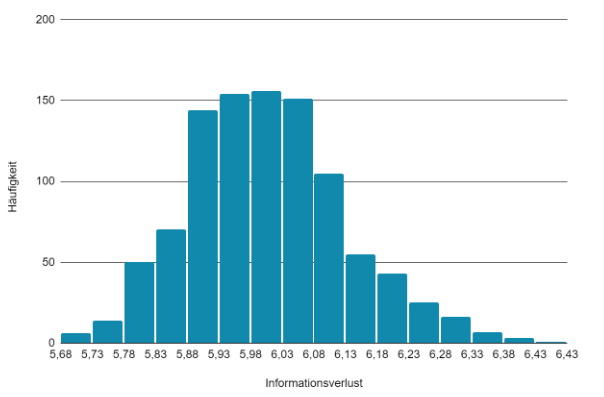
\includegraphics[scale=0.4]{Images/infloss-histogram-1000runs.png}
        \caption{Histogramm der in 1.000 Durchläufen entstandenen Informationsverluste (in Prozent) bei Anonymisierung des Benchmarkdatensatzes CENSUS durch \kanonymeans mit Standardkonfiguration und $k=3$.}
        \label{fig:histogram-census}
    \end{figure}
\end{frame}

\section{kAnonyMeans*}
\subsection{Idee}
\begin{frame}{Idee}
\begin{itemize}
    \item Zufallsfaktor: inititiale Mittelpunkte
    \item \glqq Je besser die Mittelpunkte, desto niedriger der Informationsverlust\grqq
    \item Mittelpunkte evolutionär entwickeln 
\end{itemize}
    
\end{frame}

\begin{frame}{Idee}
    \begin{figure}[h]
        \centering
        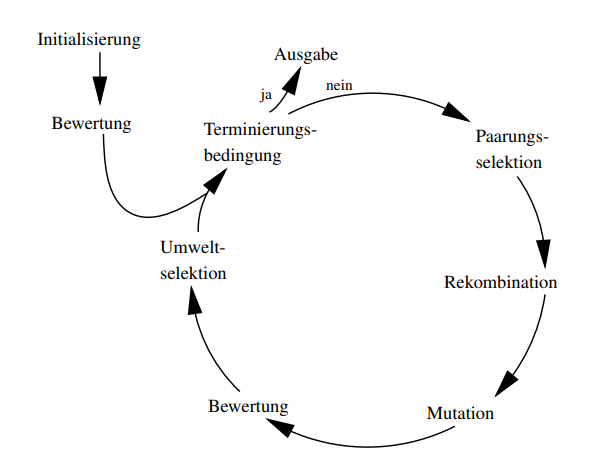
\includegraphics[scale=0.4]{Images/evoscheme.png}
        \caption{Schematische Darstellung des Zyklus bei evolutionären Algorithmen.}
        \label{fig:evoscheme}
    \end{figure}
\end{frame}

\subsection{Ausführung}
\begin{frame}{Ausführung}
    \begin{algorithm}[H]
    \renewcommand{\thealgorithm}{}
    \floatname{algorithm}{Algorithmus}
    \caption{\kanonymeansstar}
    \label{alg:kanonymeansstar}
    {\footnotesize
    \textbf{Eingabe:} Datenbank $\mathcal{X}$, Populationsgröße $p$, Überlebende $s$, Mutationen $m_c$, Mutationsstärke $m_s$\\
    \textbf{Ausgabe:} Anonymisierte Datenbank $\hat{\mathcal{X}}$ \vspace*{0.1cm}\\
    Erzeuge Startpopulation $\mathcal{M} = M_1,...,M_p$ mit $M\subseteq \mathcal{X}$ nach \forgy- oder \kmeansplusplus-Methode;\\
    Berechne $L_{\kanonymeans_{M}}(\mathcal{X})$ für alle $M \in \mathcal{M}$;\\
    \textbf{Solange} $\lnot\,$\textit{Abbruchbedingung}\\
    \hspace*{1cm}Sortiere $\mathcal{M}$ aufsteigend nach $L_{\kanonymeans_{M}}(\mathcal{X})$ mit $M\in\mathcal{M}$;\\
    \hspace*{1cm}Entferne alle Individuen $M_{s+1}$ bis $M_p$, sodass die $s$ besten Individuen überleben;\\
    \hspace*{1cm}Erzeuge aus den überlebenden Individuen (Eltern) $p-s$ neue Individuen (Kinder) \\
    \hspace*{1.5cm}und füge diese an $\mathcal{M}$ an;\\
    \hspace*{1cm}Tausche von $m_c$ Kindern jeweils $m_s$ zufällige Mittelpunkte durch zufällige Elemen-\\
    \hspace*{1.5cm}te aus $\mathcal{X}$ aus;\\
    \hspace*{1cm}Berechne $L_{\kanonymeans_{M}}(\mathcal{X})$ für alle Kinder $M \in \{M_{s+1},...,M_p\} \in \mathcal{M}$;\\
    Sortiere $\mathcal{M}$ aufsteigend nach $L_{\kanonymeans_{M}}(\mathcal{X})$ mit $M\in\mathcal{M}$;\\
    Berechne $\kanonymeans_{M_{1}}(\mathcal{X})$;\vspace*{0.1cm}
    }
    \end{algorithm}  
\end{frame}

\subsection{Ergebnisse}
\begin{frame}{Ergebnisse}
Verwendete Datensätze
\begin{itemize}
    \item Etablierte Benchmark-Datensätze
    \begin{itemize}
        \item CENSUS
        \item EIA
        \item TARRAGONA
    \end{itemize}
    \item Synthetisch generierte Datensätze
    \begin{itemize}
        \item SimU
        \item SimC
    \end{itemize}
    \item Sonstige Datensätze
    \begin{itemize}
        \item Cloud1
        \item Cloud2
    \end{itemize}
\end{itemize}
\end{frame}

\iffalse
\begin{frame}{Ergebnisse}
    \begin{figure}[H]
        \centering
        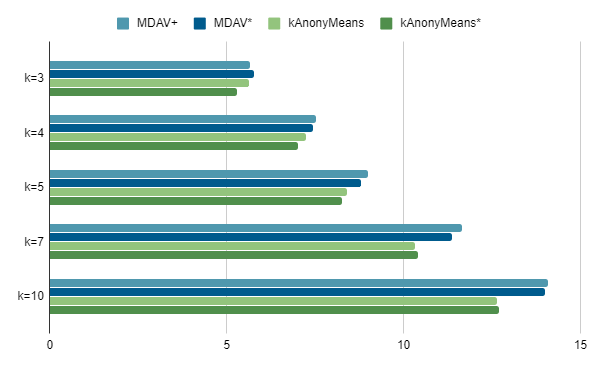
\includegraphics[scale=0.35]{Images/kAnonyMeansStarCENSUS.png}
        \caption{Informationsverluste (in Prozent) bei Anonymisierung des CENSUS Datensatzes durch verschiedene Algorithmen für verschiedene $k$.}
    \end{figure}
\end{frame}
\fi

\begin{frame}{Ergebnisse}
    \begin{figure}[H]
        \centering
        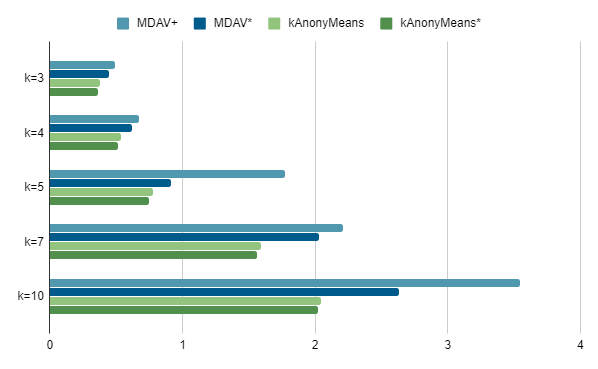
\includegraphics[scale=0.35]{Images/kAnonyMeansStarEIA.png}
        \caption{Informationsverluste (in Prozent) bei Anonymisierung des EIA Datensatzes durch verschiedene Algorithmen für verschiedene $k$.}
    \end{figure}
\end{frame}

\iffalse
\begin{frame}{Ergebnisse}
    \begin{figure}[H]
        \centering
        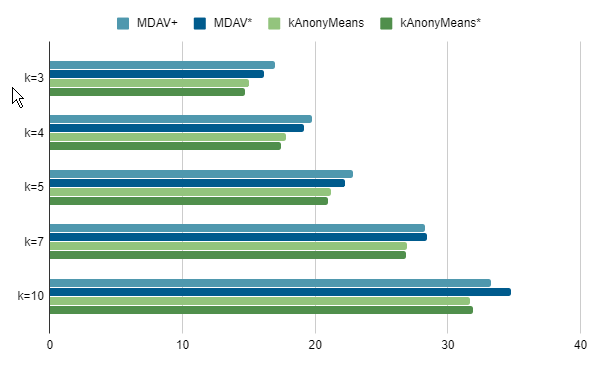
\includegraphics[scale=0.35]{Images/kAnonyMeansStarTARRAGONA.png}
        \caption{Informationsverluste (in Prozent) bei Anonymisierung des TARRAGONA Datensatzes durch verschiedene Algorithmen für verschiedene $k$.}
    \end{figure}
\end{frame}
\fi

\begin{frame}{Ergebnisse}
    \begin{figure}[H]
        \centering
        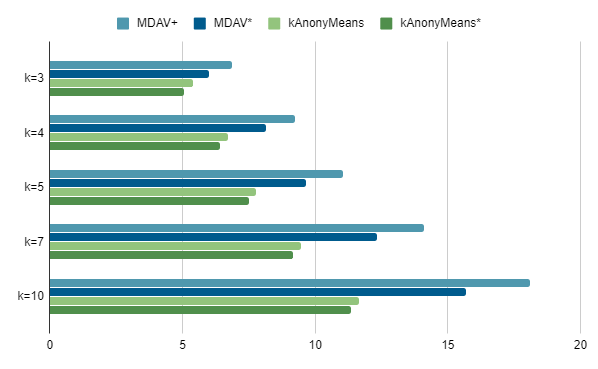
\includegraphics[scale=0.35]{Images/kAnonyMeansStarSimC.png}
        \caption{Informationsverluste (in Prozent) bei Anonymisierung des SimC Datensatzes durch verschiedene Algorithmen für verschiedene $k$.}
    \end{figure}
\end{frame}

\section{Zusammenfassung und Ausblick}
\begin{frame}{Zusammenfassung}
    \begin{itemize}
        \item \kanonymeansstar im Schnitt 17,4\% besser als \mdavplus
        \item \kanonymeansstar im Schnitt 11,6\% besser als \mdavstar
        \item \kanonymeansstar im Schnitt 3\% besser als \kanonymeans
        \item Stark auf geclusterten Daten
        \item Je größer $k$, desto stärker \kanonymeans
    \end{itemize}
\end{frame}

\begin{frame}{Ausblick - kAnonyMeans}
    \begin{itemize}
        \item Zufallsabhängikeiten minimieren
        \item optimale Paramterbelegung finden
        \item bessere Rekombinations- / Mutationsstrategien
    \end{itemize}
\end{frame}

\begin{frame}{Ausblick - Mikroaggregation}
    \begin{itemize}
        \item Optimaler Algorithmus
        \item besserer Approximationsalgorithmus als $\mathcal{O}(k^3)$
        \item Linearzeitalgorithmus
        \item Mikroaggregation durch evolutionäre Strategie
    \end{itemize}
\end{frame}

\nocite{*}
\appendix
\begin{frame}[noframenumbering, plain]
\Large\center
Danke für Ihre Aufmerksamkeit!
\end{frame}

\begin{frame}[noframenumbering]{MDAV}
    \begin{algorithm}[H]
    \renewcommand{\thealgorithm}{}
    \floatname{algorithm}{Algorithmus}
    \caption{\mdavplus}
    \label{alg:mdavplus}
    {
    \textbf{Eingabe:} Datenbank $\mathcal{X}$, Anonymitätsparameter $k$ \\
    \textbf{Ausgabe:} $k$-anonyme Datenbank $\hat{\mathcal{X}}$
    \begin{enumerate}
        \item Berechne den Schwerpunkt $c(\mathcal{X})$ der Eingabedatenmenge $\mathcal{X}$.
        \item Wähle jenen noch nicht zugewiesenen Eintrag $\mathbf{x} \in \mathcal{X}$, der am weitesten von $c(\mathcal{X})$ entfernt ist.
        \item Bilde eine Gruppe um $\mathbf{x}$ bestehend aus $\mathbf{x}$ und seinen $k-1$ nächsten nicht zugewiesenen Nachbarn (diese Elemente sind nun zugewiesen).
        \item Wenn mindestens $k$ nicht zugewiesene Einträge übrig sind, gehe zurück zu Schritt 2, andernfalls weise alle noch nicht zugewiesenen Elemente der zu ihnen nächsten Gruppe zu.
    \end{enumerate}\vspace*{0.1cm}
    }
    \end{algorithm}
\end{frame}

\begin{frame}[noframenumbering]{k-means}
    Auswahl der initialen Mittelpunkte
    \begin{itemize}
        \item \forgy
        \item \kmeansplusplus
    \end{itemize}
\end{frame}

\begin{frame}[noframenumbering]{Laufzeit und Informationsverlust bei kAnonyMeans}
    \begin{figure}[H]
        \centering
        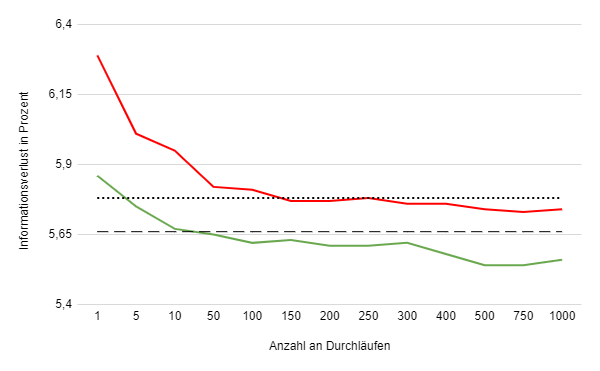
\includegraphics[scale=0.45]{Images/kanonymeansminmax.png}
        \caption{\footnotesize Minimaler (grüne Linie) und maximaler (rote Linie) Informationsverlust (in Prozent) bei fünfzigmal durchgeführter Anonymisierung des CENSUS-Datensatzes mittels \kanonymeans für $k=3$ bei verschiedener Anzahl an Durchläufen. Die gepunktete Linie gibt zum Vergleich den Informationsverlust bei Verwendung von \mdavstar an, die gestrichelte Linie den von \mdavplus.}
    \end{figure}
\end{frame}

\begin{frame}[noframenumbering]{Laufzeit und Informationsverlust bei kAnonyMeans*}
    \begin{figure}[H]
        \centering
        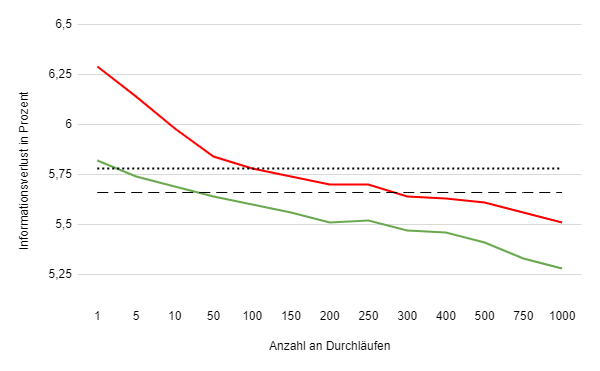
\includegraphics[scale=0.45]{Images/kanonymeansstarminmax.png}
        \caption{\footnotesize Minimaler (grüne Linie) und maximaler (rote Linie) Informationsverlust (in Prozent) bei fünfzigmal durchgeführter Anonymisierung des CENSUS-Datensatzes mittels \kanonymeansstar für $k=3$ bei verschiedener Anzahl an Durchläufen. Die gepunktete Linie gibt zum Vergleich den Informationsverlust bei Verwendung von \mdavstar an, die gestrichelte Linie den von \mdavplus.}
    \end{figure}
\end{frame}

\begin{frame}[allowframebreaks, noframenumbering]{References}
        \bibliographystyle{amsalpha}
        \bibliography{lit.bib}
\end{frame}

\end{document}
